%% Начало содержательной части.
\chapter{Практическое исследование}

В данной главе речь пойдет об анализе данных.
Рассматривается практическая сторона решения.
Рассказывается про классы наборов данных, которые использовались.
Приведены результаты классификации новых датасетов по имеющейся информации об известных.

\section{Классы исследования}

На данный момент в компании <<VeeRoute>> данных не так много.
Они будут появляться со временем.
Для исследования брались 4 разных класса наборов данных, практически никак не связанных друг с другом.

В исследовании участвовали следующие классы:

\begin{itemize}
	\item Norway;
 	\item Gulfstream;
	\item Austria;
	\item DelLine.
\end{itemize}

\subsection{Класс Norway}

\begin{enumerate}
\item Норвежские бенчмарки
\item Были сгенерированы автоматически
\item Класс связан с задачей Delivery	

\end{enumerate}

\subsection{Класс Gulfstream}

\begin{enumerate}
	\item Данные по гольфстриму
	\item Сервисное обслуживание / обслуживание объектов
	\item Москва и Московская область
\end{enumerate}


\subsection{Класс Austria}

\begin{enumerate}
	\item Данные почты Австрии
	\item Класс связан с задачей Pickup and Delivery
	\item Широкие и узкие окна в одном файле на разные даты
\end{enumerate}

\subsection{Класс DelLine}

\begin{enumerate}
	\item Москва
	\item Класс связан с задачей Pickup and Delivery
	\item Деловые линии, под платформу <<VeeRoute>>, 5489 заказов
\end{enumerate}


\section{Машинное обучение в данной задаче}

В каждом классе выбиралось одинаковое числов наборов для рассмотрения (10).
В качестве обучающей выборки бралось ~--- 50 \% от каждого класса наборов данных.
В качестве тестовой выборки ~--- 50 \% оставшихся данных.
При каждом запуске данные перемешивались.

Стоит также отметить,что наборы данных для всех классов, кроме Norway, были получены из одного большого датасета, путем семплирования.
Каждый большой набор данных соответственно делился на много маленьких.

\textbf{Определение.} Истинно-положительные (true positives) --- те объекты, которые должны были быть определены и определились на выходе.

\textbf{Определение.} Ложно-положительные (false positives) --- те объекты, которые не должны были быть определены, но анализатор их вернул на выходе.

\textbf{Определение.} Ложно-отрицательные (false negatives) --- те объекты, которые должны были быть определены, но их не вернули на выходе.

\textbf{Определение.} Истинно-отрицательные (true negatives) --- объекты, которых быть на выходе не должно и анализатора их совершенно правильно не вернул.

\textbf{Определение.} Истинно-отрицательные (true negatives) --- объекты, которых быть на выходе не должно и анализатора их совершенно правильно не вернул.

Определим меру точности как:
\[precision = \frac{tp}{tp+ fp}\]

Определим меру полноты как:
\[recall = \frac{tp}{tp+ fn}\]

\textbf{Определение.}  $F_1$ мера --- среднее гармоническое величин
$precision$  и $recall$.
\[F_1 = 2 * \frac{precision*recall}{precison+ recall}\]


\section{Результаты работы программы}

Для классификации использовалась утилита Weka. Тестовые и обучающие выборки представлены в формате ARFF.
Файлы включает в себя заголовок с типами (в данном случае, с числовыми) и информационную секцию со значениями по каждому признаку.
Также указано количество классов, на которые будет происходить классификация (входит в заголовок).

В таблицах приведены результаты пяти запусков, каждый раз выборки менялись.
В левом столбце указаны типы классификаций, в верхней строчке указываются прогоны и среднее арифметическое по всем запускам в этой категории.

Благодаря этому тестированию, можно будет понимать, какой тип классификации наилучшим образом работает с данной задачей.

Очень важно также  понимать, какой ключевой фактор определения принадлежности к тому или иному классу.
То есть, какие признаки чаще всего <<классифицируют>> датасеты.

\subsection{Все признаки используются}
 
\begin{table}[!h]
	\centering
	\caption{Все признаки используются}\label{tab1}
	\begin{tabu}{|*{18}{c|}}\hline
		    &  1  & 2 & 3 & 4 & 5 & Среднее \\\hline
		Дерево Решений & 0.949 & 0.949 & 0.949  & 0.949 & 0.949 & 0.949 \\\hline
		SVM &  0.949 & 0.949 & 0.949  & 0.949 & 0.949 & 0.949 \\\hline
		LogReg & 0.949 & 0.949 & 0.949  & 0.949 & 0.949 & 0.949  \\\hline
		RandomForest &0.903 & 0.949 & 0.903 &  0,852  & 0.949 & 0.911 \\\hline
	\end{tabu}
\end{table}

В целом, опираясь на таблицу~\ref{tab1}, можно сказать,что все типы, за исключением Random Forest, показали отличный результат.
С помощью <<Деревьев Решений>> можно внимательно оценить, какие признаки влияли на результат.
\begin{figure}[h]
	\caption{<<Дерево решений>> в случае со всеми признаками \label{tree1}} \centering
	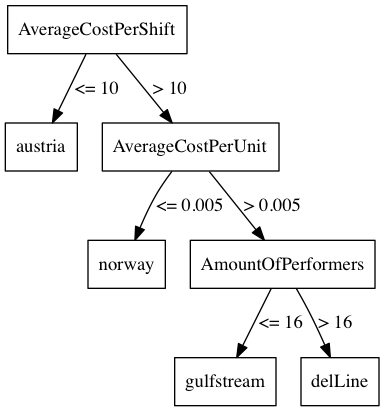
\includegraphics[scale=0.70]{tree1}
\end{figure}

Как видно из рисунка~\ref{tree1} , ключевыми признаками являются:
\begin{itemize}
\item $AverageCostPerShift$ / Средняя цена за использование смены исполнителем или транспортом 
\item $AverageCostPerUnit$ / Средняя цена за минуту (для исполнителя), метр (для транспорта)
\item $AmountOfPerformers$ / Количество исполнителей заказов
\end{itemize}

\subsection{Убираются три признака при построении классификатора}

Очень важно иногда убирать признаки, при тестировании, чтобы посмотреть, как поведет себя $F_1$ мера.
Некоторые признаки могут отрицательно влиять на классификацию.
На самом деле, отрицательно --- не значит плохо.
Просто если какой-то признак будет постоянно являться ключевым при определении принадлежности к тому или иному датасету, то это не совсем хорошо, поскольку важно собрать, как можно больше  различных признаков, которые будут являться ключевыми при классификации.
Например, в предыдущем пункте указаны признаки, по которым, если внедрить какие-нибудь данные из реальной жизни, классификатор не будет к этому готов.
Имеет место переобучение.

Далее мы <<зашумим>> три признака, которые влияли на результат в прошлой подглаве.

\begin{table}[!h]
	\centering
	\caption{Не используется признаки количества водителей, средняя цена за использование смены исполнителем или транспортом, средняя цена за минуту (для исполнителя), метр (для транспорта) }\label{tab2}
			\begin{tabu}{|*{18}{c|}}\hline
			                           &  1  & 2 & 3 & 4 & 5 & Среднее \\\hline
			Дерево Решений & 1.000 & 0.949 & 1.000  & 0.949 & 0.949 & 0.969 \\\hline
			SVM                    &  1.000 & 0.949 & 1.000  & 0.949 & 0.949 & 0.969 \\\hline
			LogReg              & 0.949 & 0.949 & 1.000  & 0.949 & 0.899 & 0.949  \\\hline
			RandomForest &1.000 & 0.949 & 1.000 &  0,949  & 0.949 & 0.969 \\\hline
		\end{tabu}
\end{table}

В целом, опираясь на таблицу~\ref{tab2}, можно сказать,что все типы показали отличный результат.
Чуть хуже повела себя логистическая регрессия.

\begin{figure}[h]
	\caption{<<Дерево решений>> в случае с 3 зашумленными признаками \label{tree2}} \centering
	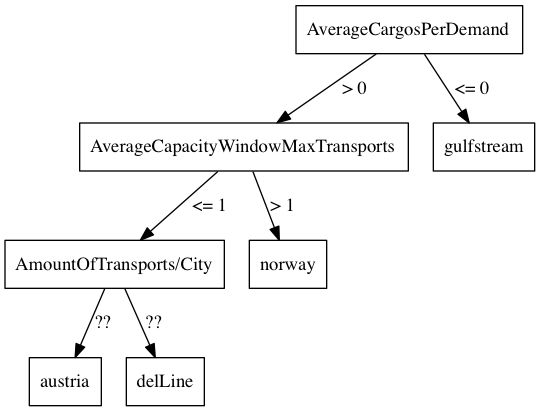
\includegraphics[scale=0.70]{tree2}
\end{figure}

Как видно из рисунка~\ref{tree2} , ключевыми признаками являются:

\begin{itemize}
	\item $AverageCargosPerDemand $ / Среднее количество грузов в заказах
	\item $AverageCapacityWindowMaxTransports$ / Количество транспорта, который может работать в локации одновременно
\end{itemize}

Собственно $AverageCargosPerDemand $ действительно очень правильно определяет класс \textit{gulfstream}, так он очень существенно выделяется количеством грузов в заказах.
$AverageCapacityWindowMaxTransports$ чаще всего пишется тестировщиками, так что по этому признаку очень тяжело судить, его можно отбросить.

\subsection{<<Зашумляется>> еще один признак при построении классификатора}

Далее исследование продолжается без четырех признаков, рассматриваемых выше.

\begin{table}[!h]
	\centering
	\caption{Не используются 4 признака, указанных выше в подглавах $3.3.1$ и $3.3.2$}\label{tab3}
	\begin{tabu}{|*{18}{c|}}\hline
	                          &  1  & 2 & 3 & 4 & 5 & Среднее \\\hline
	Дерево Решений & 1.000 & 0.949 & 1.000  & 1.000 & 0.949 & 0.980 \\\hline
	SVM                    &  1.000 & 0.949 & 1.000  & 1.000 & 0.949 & 0.980 \\\hline
	LogReg              & 0.949 & 0.949 & 1.000  & 1.000 & 0.949 & 0.969  \\\hline
	RandomForest &    0.949 & 0.949 & 0.949 &  0.949  & 0.899 & 0.940 \\\hline
\end{tabu}
\end{table}

Опираясь на таблицу~\ref{tab3}, можно заметить,что результаты на всех типа показаны одинаково неплохие.

\begin{figure}[h]
	\caption{Первый из встречающихся вариантов <<Дерева решений>> в случае с 4 <<зашумленными>> признаками \label{tree3}} \centering
	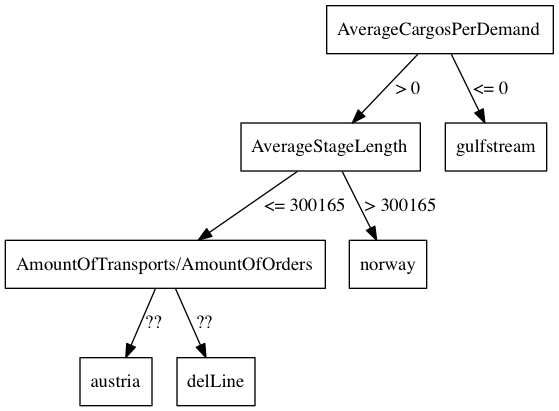
\includegraphics[scale=0.70]{tree3}
\end{figure}

\begin{figure}[h]
	\caption{Второй из встречающихся вариантов <<Дерева решений>> в случае с 4 <<зашумленными>> признаками \label{tree4}} \centering
	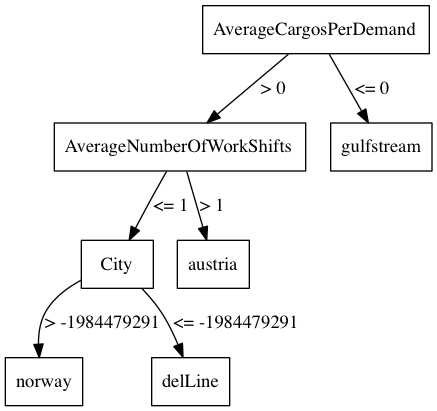
\includegraphics[scale=0.70]{tree4}
\end{figure}

Как видно из рисунка~\ref{tree3} и рисунка~\ref{tree4} , ключевыми признаками в данном случае чаще всего являлись:
\begin{itemize}
	\item $AverageStageLength$ / Средняя длительность временного отрезка в минутах (для исполнителя), длительность пути в метрах (для транспорта)
	\item $AverageNumberOfWorkShifts$ / Среднее количество рабочих смен для исполнителей
	\item $AmountOfOrders$ / Количество заказов
	\item $AmountOfTransports$ / Количество транспортых средств, выполняющих заказы
	\item $City$ / Город, где проводится доставка
\end{itemize}

Первый признак действительно грамотный для определения класса \textit{norway}, второй хорошо идентифицирует класс \textit{austria}.

Про последние 3 признака и их не слишком большую информативность, речь пойдет в следующем разделе.

\subsection{Дополнительные прогоны}

Признаки $AmountOfOrders$, $AmountOfTransports$, $City$ на тех данных, на которых происходит исследование, могут давать не всегда информативные результаты.Во многом, это связано со спецификой семплирования. К тому же город тоже очень сильно может перетягивать одеяло на себя по той причине, что данных очень мало, и регионы в датасетах практически все различные.

Попробуем посмотреть,что получится, если <<зашумить>> все неинформативные признаки, и те, что указаны в этом разделе.

\begin{table}[!h]
	\centering
	\caption{Дополнительные прогоны с <<зашумлением>> неинформативных признаков }
	\label{tab4}
			\begin{tabu}{|*{18}{c|}}\hline
			&  1  & 2 & 3 & 4 & 5 & Среднее \\\hline
			Дерево Решений & 1.000 & 0.949 & 0.949  & 1.000 & 1.000 & 0.980 \\\hline
			SVM                    &  0,949  & 0,949  & 0.949  & 1.000 & 0.949 & 0.960 \\\hline
			LogReg              & 0.675 & 0.764 & 0.804  & 0.709 & 0.719 & 0.734  \\\hline
			RandomForest    &   0,899  & 0,896 & 0.899 &  1.000 & 0.949 & 0.929 \\\hline
		\end{tabu}
\end{table}

Можно обратить внимание, на то, что на этих прогонах сильно <<просела>> LogReg, как и Random Forest.
Лучший результат показало <<Дерево Решений>>.

 Признаки чаще всего определялись из того множества, что было указано в предыдущих разделах.
 Без многих неинформативных признаков ключевыми также стали features, посчитанные по матрицам совместимости.
 Пример <<точного>> решения представлен на рисунке~\ref{tree5}.
 Здесь $F_1$ мера постоянно равнялась 1, на нижнем уровне менялись признаки, но они всегда относились к категории <<матрицы совместимости>>.

\begin{figure}[h]
	\caption{Пример <<Дерева Решений>>, в котором присутствуют признаки <<матрицы совместимости>> \label{tree5}} \centering
	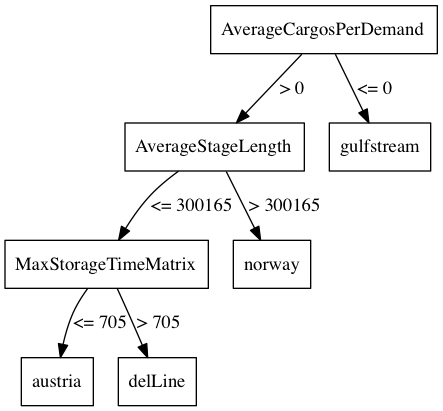
\includegraphics[scale=0.68]{tree5}
\end{figure}


\chapterconclusion

В данной главе речь идет об анализе данных, рассматривается практическая сторона решения.
Рассказывается про классы наборов данных, которые были рассмотрены.
Высчитывается метрика на нескольких моделях, выделяются ключевые признаки, делаются выводы.
Как можно заметить, лучший результат в среднем показывается при <<Дереве Решений>>.
Усредненная $F_1$ мера составляет 0.967.

